\subsection{}
\begin{tabular}{llll}
$VC(\phi_{01}=(1,0,0,0)$&$VC(\phi_{11}=(1,1,0,0)$&$VC(\phi_{21}=(0,0,1,0)$&$VC(\phi_{31}=(0,0,0,1)$\\
$VC(\phi_{02}=(2,0,0,0)$&$VC(\phi_{12}=(1,2,1,0)$&$VC(\phi_{22}=(0,0,2,1)$&$VC(\phi_{32}=(2,0,0,2)$\\
$VC(\phi_{03}=(3,3,1,0)$&$VC(\phi_{13}=(1,3,1,0)$&$VC(\phi_{23}=(2,0,3,3)$&$VC(\phi_{33}=(2,0,0,3)$\\
$VC(\phi_{04}=(4,3,1,4)$&$VC(\phi_{14}=(1,4,1,0)$&$VC(\phi_{24}=(5,3,4,4)$&$VC(\phi_{34}=(2,0,0,4)$\\
$VC(\phi_{05}=(5,3,1,4)$&$VC(\phi_{15}=(5,5,5,4)$&$VC(\phi_{25}=(5,3,5,4)$&$VC(\phi_{35}=(2,4,1,5)$\\
$VC(\phi_{06}=(6,3,1,4)$&$VC(\phi_{16}=(5,6,5,6)$&$VC(\phi_{26}=(6,3,6,4)$&$VC(\phi_{36}=(2,4,1,6)$\\
\end{tabular}
\subsection{}
Bei den Ereignissen $\phi_{34}, \phi_{04}, \phi_{24}$ und $\phi_{15}$ gilt\\
$\phi_{34}\ vor\ \phi_{04}\ vor\ \phi_{24}\ vor\ \phi_{15}$ mit\\
$(2,0,0,4)_{\phi_{34}} < (4,3,1,4)_{\phi_{04}} < (5,3,4,4)_{\phi_{24}} < (5,5,5,4)_{\phi_{15}}$.
\subsection{}
Die Ereignisse $\phi_{11}, \phi_{02}, \phi_{21}, \phi_{31}$ sind paarweise unabhängig:
$(1,1,0,0)_{\phi_{11}} || (2,0,0,0)_{\phi_{02}} || (0,0,1,0)_{\phi_{21}} || (0,0,0,1)_{\phi_{31}}$.
\subsection{}
\subsection{}
Der Präzedenzgraph ist praktisch bereits auf dem Zettel angegeben.
\subsection{}
Folgendes Petrinetz haben wir zu dem gegebenem Zeitskalenmodell angefertigt:
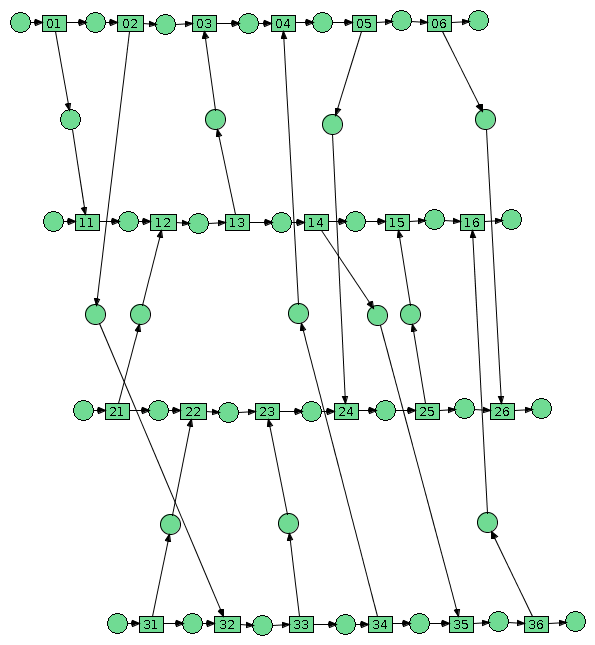
\includegraphics[scale=0.5]{./b06_a636.png}